\chapter{JSON, XML, and YAML}\label{json-xml-and-yaml}

\section{Data Serialization}\label{data-serialization}

\begin{itemize}
\tightlist
\item
  DATA SERIALIZATION is the process of converting DATA into a
  standardized format/structure that can be stored (in a file) or
  transmitted (over a network) and reconstructed later (ie: by a
  different application)

  \begin{itemize}
  \tightlist
  \item
    This allows the DATA to be communicated between applications in a
    way both APPLICATIONS understand.
  \end{itemize}
\item
  DATA SERIALIZATION languages allow us to represent \emph{variables}
  with text
\end{itemize}

\begin{figure}
\centering
\pandocbounded{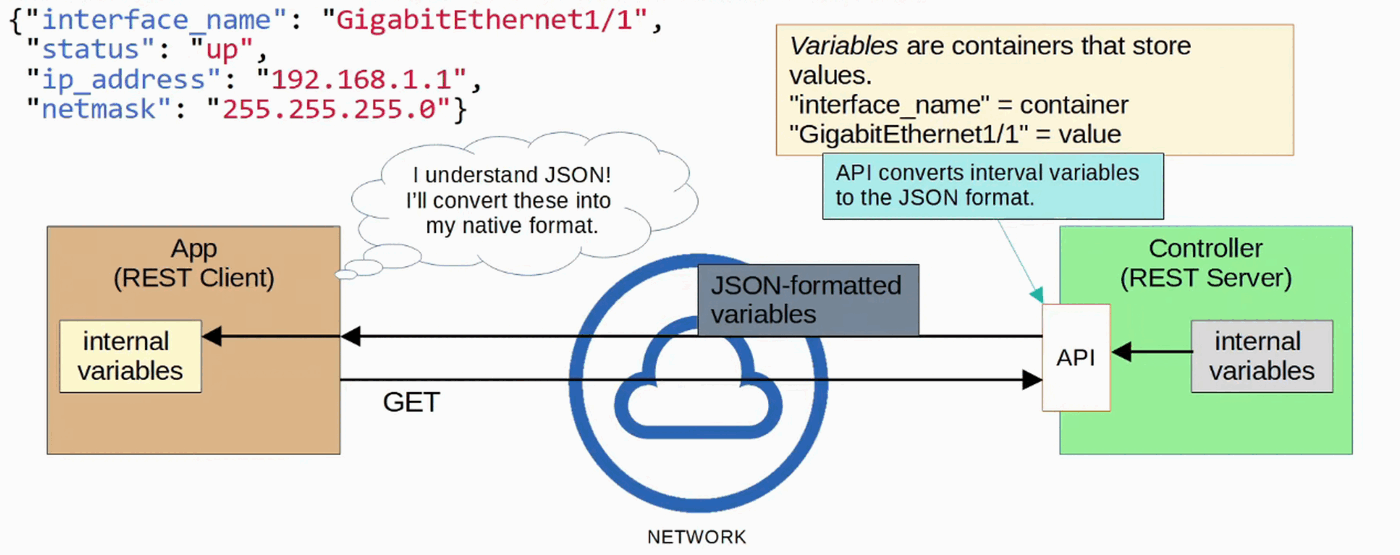
\includegraphics[keepaspectratio,alt={image}]{images/63-json-xml-yaml/img-001.png}}
\end{figure}

\section{JSON (Javascript Object
Notation)}\label{json-javascript-object-notation}

\begin{itemize}
\item
  JSON (JAVASCRIPT OBJECT NOTATION) **is an open standard FILE FORMAT
  and DATA INTERCHANGE FORMAT that uses human-readable text to store and
  transmit data objects
\item
  It is standardized in RFC 8259
  (\url{https://datatracker.ietf.org/doc/html/rfc8259})
\item
  It was derived from JavaScript, but it is language-independent and
  many modern programming languages are able to generate and read JSON
  data

  \begin{itemize}
  \tightlist
  \item
    REST APIs often use JSON
  \end{itemize}
\item
  \emph{Whitespace} is insignificant
\item
  JSON can represent FOUR ``primitive'' DATA Types:

  \begin{itemize}
  \tightlist
  \item
    String
  \item
    Number
  \item
    Boolean
  \item
    Null
  \end{itemize}
\item
  JSON also has TWO ``structured'' DATA Types:

  \begin{itemize}
  \tightlist
  \item
    Object
  \item
    Array
  \end{itemize}
\end{itemize}

\section{JSON Primitive Data Types}\label{json-primitive-data-types}

\begin{itemize}
\tightlist
\item
  A STRING is a text value. It is surrounded by double quotes `` ``

  \begin{itemize}
  \tightlist
  \item
    ``Hello''
  \item
    ``Five''
  \item
    ``5''
  \end{itemize}
\item
  A NUMBER is a numeric value. It is NOT surrounded by quotes

  \begin{itemize}
  \tightlist
  \item
    5
  \item
    100
  \end{itemize}
\item
  A BOOLEAN is a DATA Type that has only TWO possible values, not
  surrounded by quotes

  \begin{itemize}
  \tightlist
  \item
    true
  \item
    false
  \end{itemize}
\item
  A NULL value represents the intentional absence of any object value.
  It is not surrounded by quotes

  \begin{itemize}
  \tightlist
  \item
    null
  \end{itemize}
\end{itemize}

\section{JSON Structured Data Types}\label{json-structured-data-types}

\begin{itemize}
\tightlist
\item
  An OBJECT is an unordered list of \emph{key-value pairs} (variables)

  \begin{itemize}
  \tightlist
  \item
    Sometimes called a DICTIONARY
  \item
    OBJECTS are surrounded by curly brackets \{\}
  \item
    The \emph{key} is a STRING
  \item
    The \emph{value} is any valid JSON DATA Type (string, number,
    boolean, null, object, array)
  \item
    The \emph{key} and \emph{value} are separated by a colon :
  \item
    If there are multiple key-value pairs, each pair is separated by a
    comma
  \end{itemize}
\end{itemize}

\begin{figure}
\centering
\pandocbounded{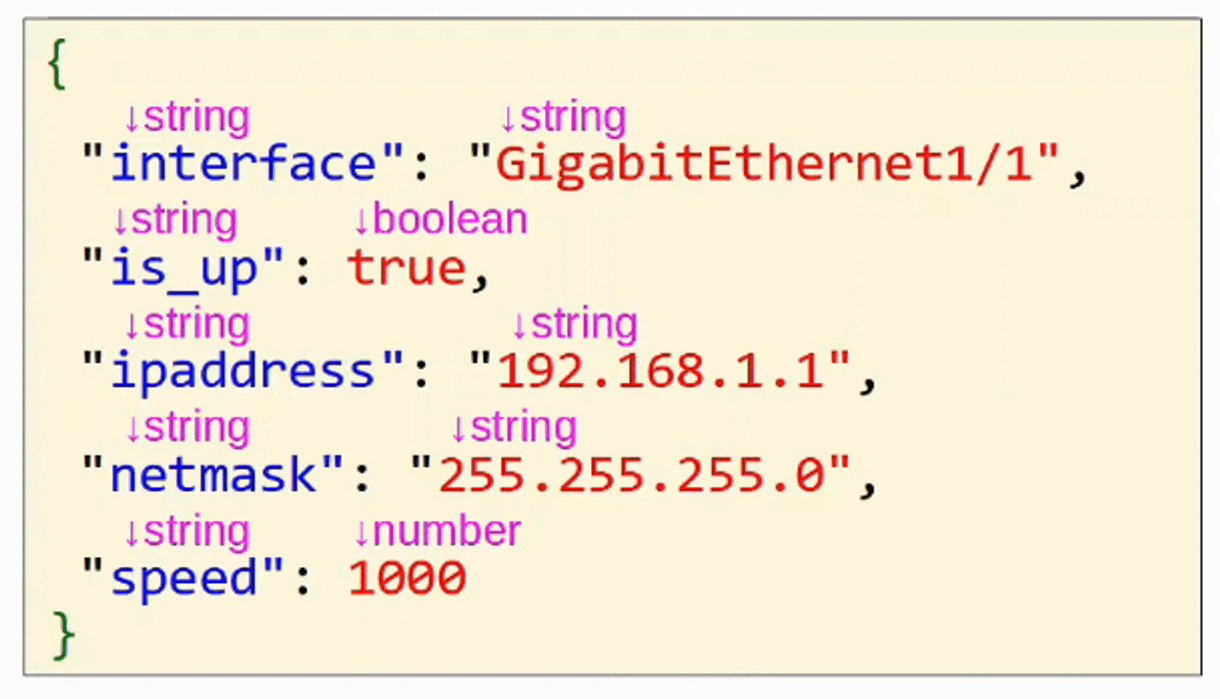
\includegraphics[keepaspectratio,alt={image}]{images/63-json-xml-yaml/img-002.png}}
\end{figure}

\begin{figure}
\centering
\pandocbounded{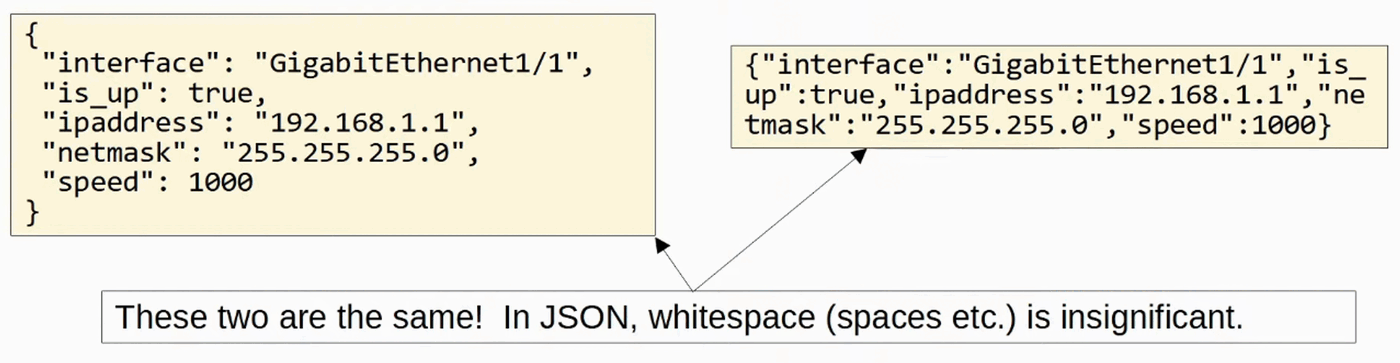
\includegraphics[keepaspectratio,alt={image}]{images/63-json-xml-yaml/img-003.png}}
\end{figure}

\begin{figure}
\centering
\pandocbounded{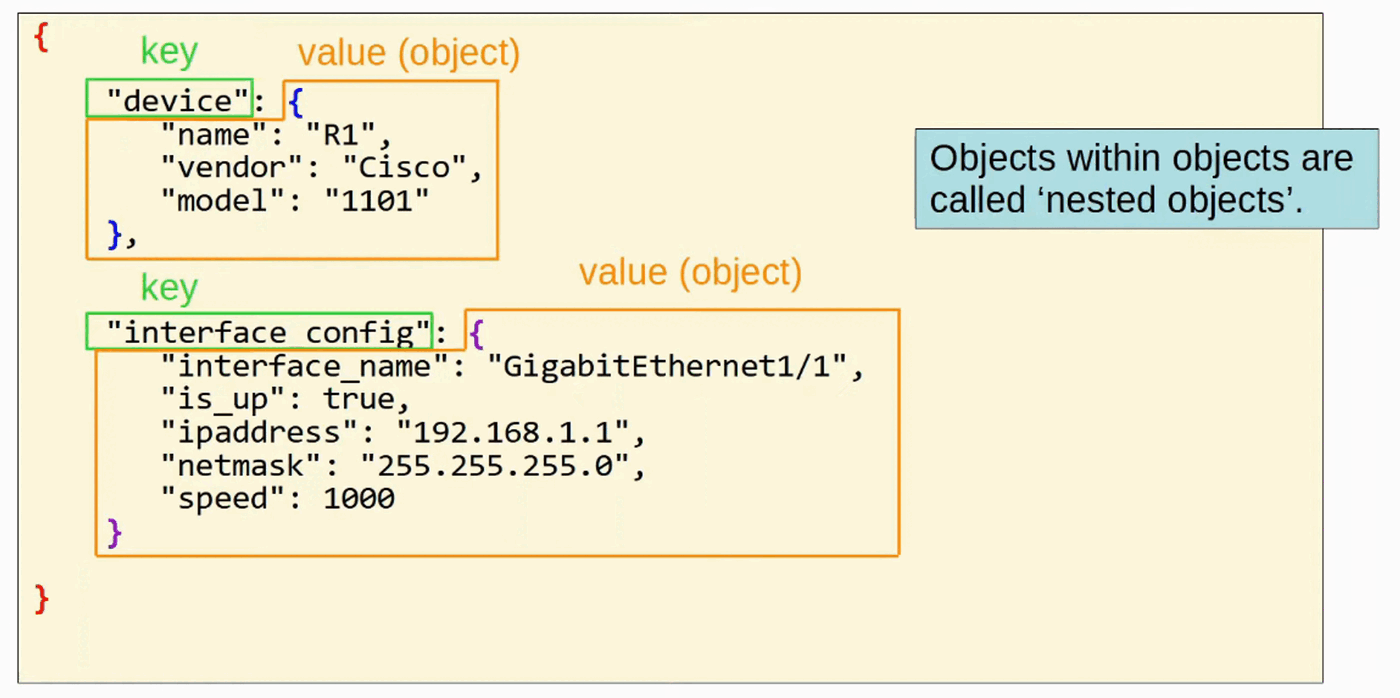
\includegraphics[keepaspectratio,alt={image}]{images/63-json-xml-yaml/img-004.png}}
\end{figure}

\begin{itemize}
\tightlist
\item
  An ARRAY is a series of \emph{values} separated by commas

  \begin{itemize}
  \tightlist
  \item
    Not \emph{key-value pairs}
  \item
    The values do NOT have to be the same DATA Type
  \end{itemize}
\end{itemize}

\begin{figure}
\centering
\pandocbounded{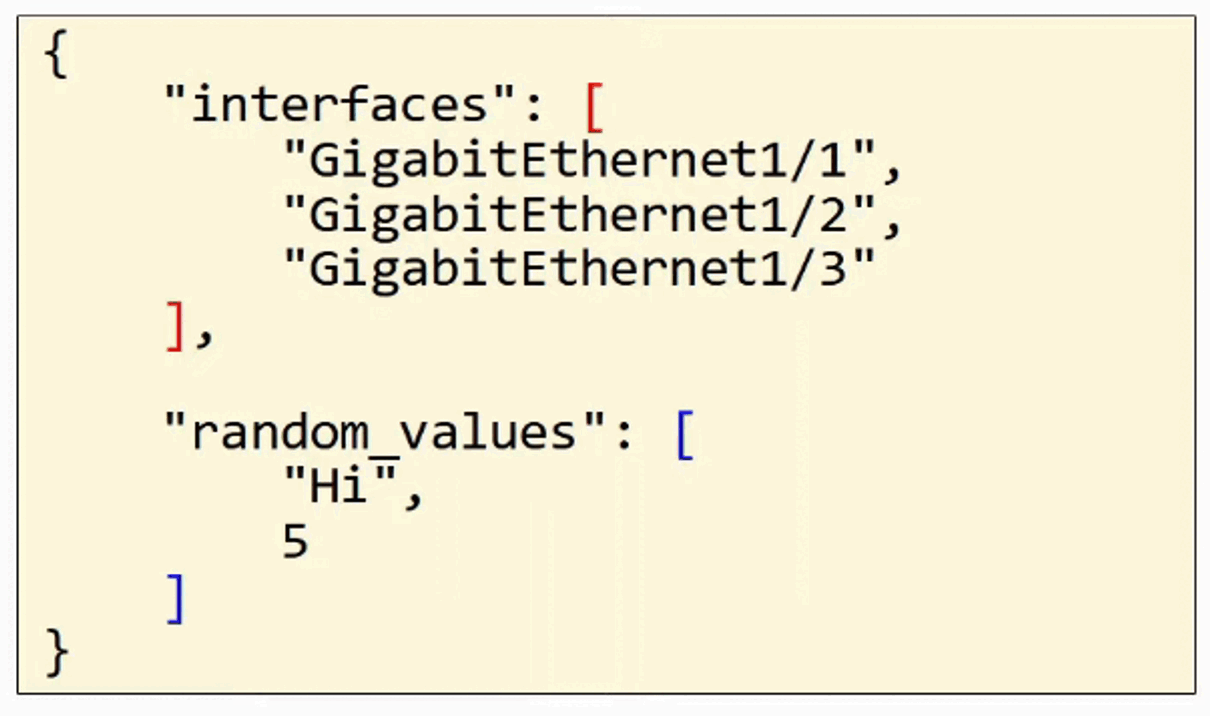
\includegraphics[keepaspectratio,alt={image}]{images/63-json-xml-yaml/img-005.png}}
\end{figure}

\begin{figure}
\centering
\pandocbounded{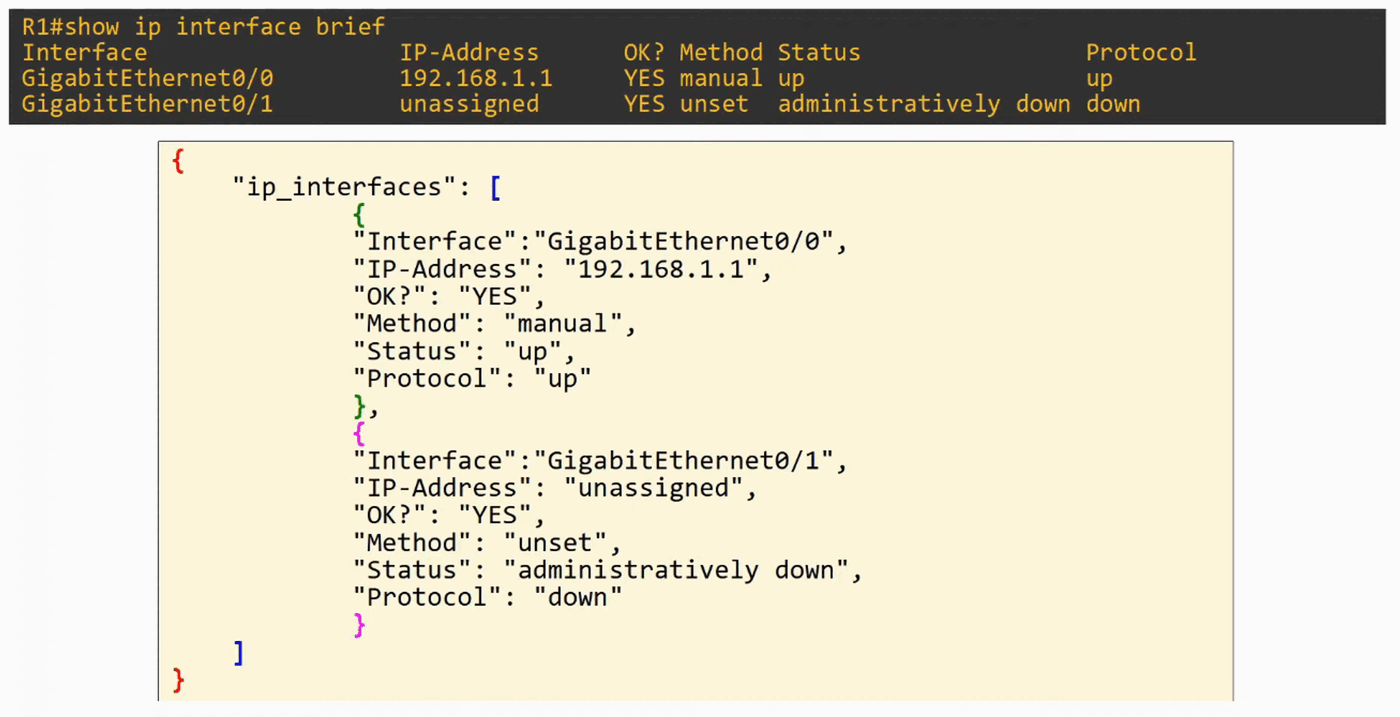
\includegraphics[keepaspectratio,alt={image}]{images/63-json-xml-yaml/img-006.png}}
\end{figure}

\section{XML (Extensible Markup
Language)}\label{xml-extensible-markup-language}

\begin{itemize}
\tightlist
\item
  XML (EXTENSIBLE MARKUP LANGUAGE) was developed as a MARKUP language,
  but is now used as a general data serialization language

  \begin{itemize}
  \tightlist
  \item
    Markup languages (ie: HTML) are used to format text (font, size,
    color, headings, etc)
  \item
    XML is generally less human-readable than JSON
  \item
    Whitespace is insignificant
  \item
    Often used by REST APIs
  \item
    \textless key\textgreater{} value \textless/key\textgreater{}
    (similar to HTML)
  \end{itemize}
\end{itemize}

\begin{figure}
\centering
\pandocbounded{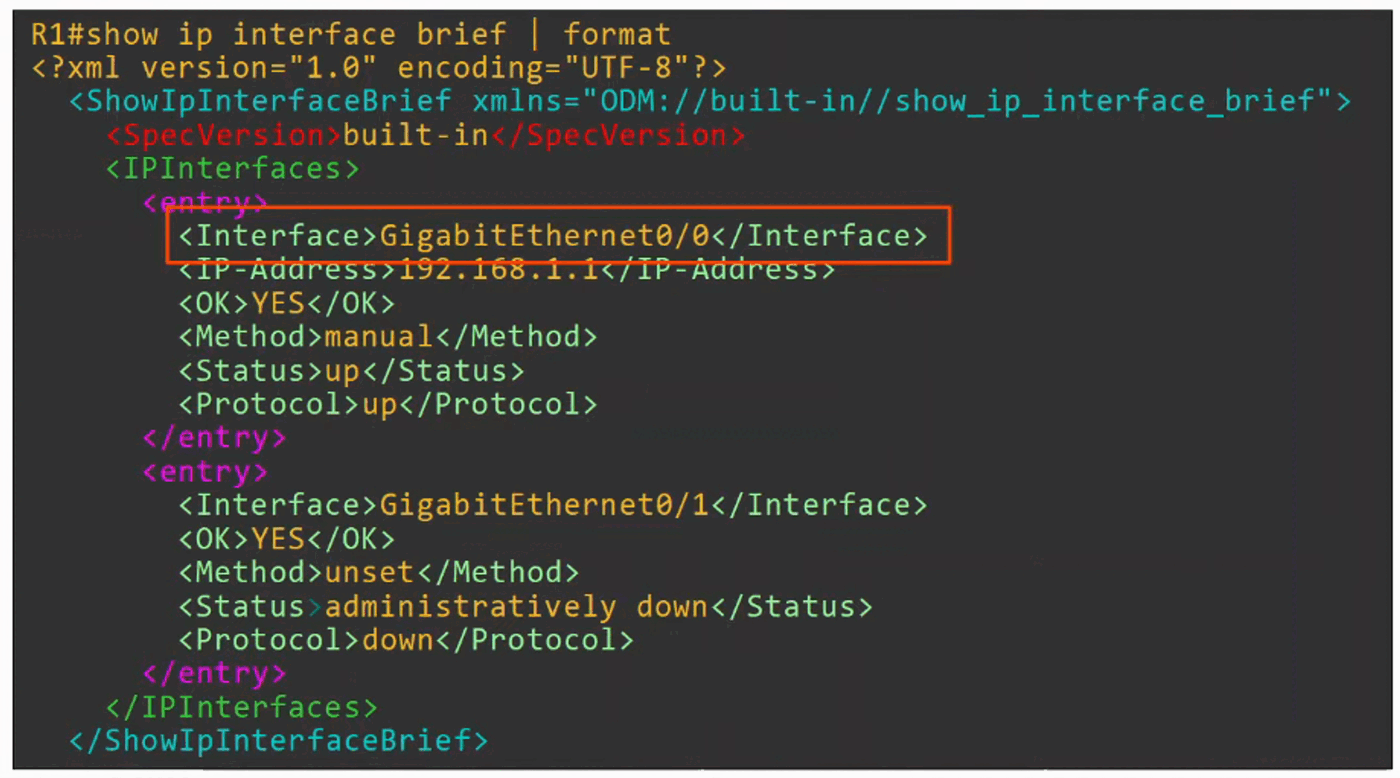
\includegraphics[keepaspectratio,alt={image}]{images/63-json-xml-yaml/img-007.png}}
\end{figure}

\begin{figure}
\centering
\pandocbounded{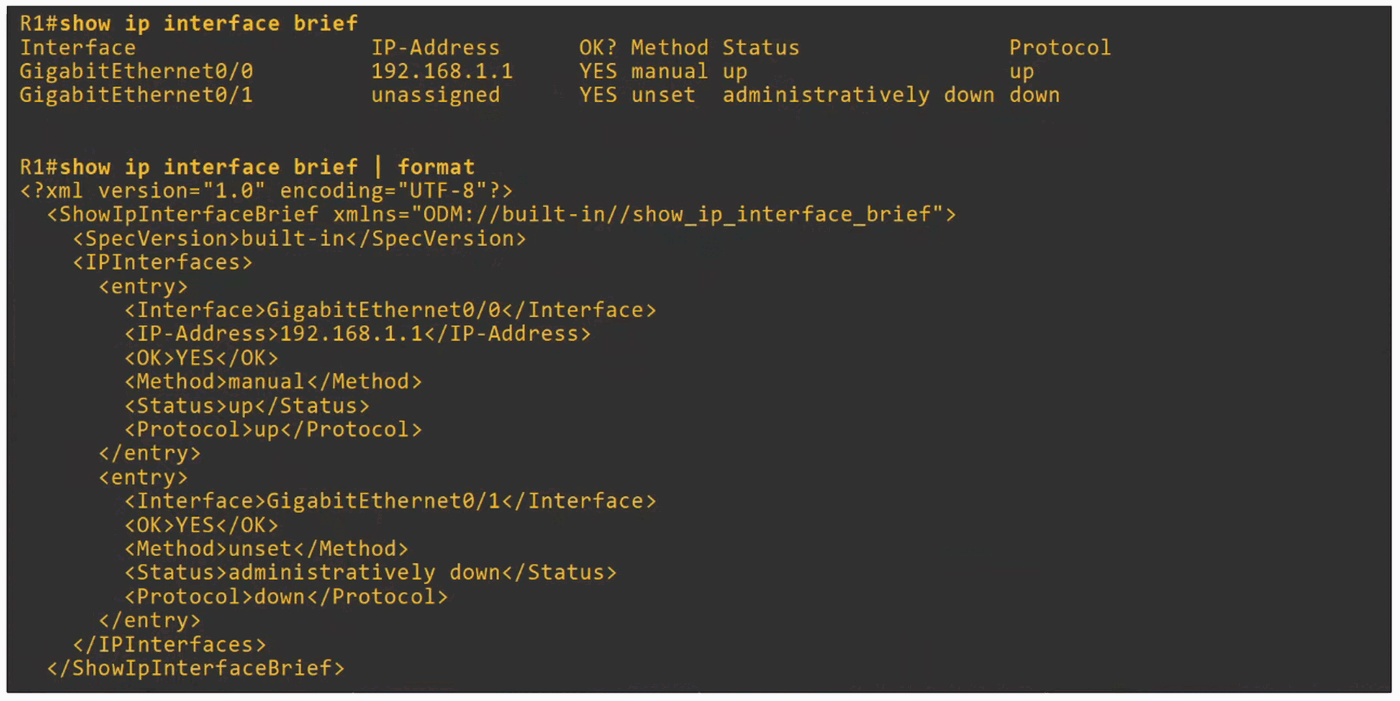
\includegraphics[keepaspectratio,alt={image}]{images/63-json-xml-yaml/img-008.png}}
\end{figure}

\section{YAML (YAML Ain't Markup
Language)}\label{yaml-yaml-aint-markup-language}

\begin{itemize}
\tightlist
\item
  YAML originally meant \emph{YET ANOTHER MARKUP LANGUAGE} but to
  distinguish its purpose as a data-serialization language rather than a
  markup language, it was repurposed to \emph{YAML AINT MARKUP LANGUAGE}
\item
  YAML is used by the network automation tool ANSIBLE (covered later in
  the course)
\item
  YAML is VERY Human-Readable
\item
  Whitespace \textbf{is significant} (unlike JSON and XML)

  \begin{itemize}
  \tightlist
  \item
    Indentation is very important
  \end{itemize}
\item
  YAML files start with - - - (three dashes)
\item
  \begin{itemize}
  \tightlist
  \item
    is used to indicate a list
  \end{itemize}
\item
  Keys and Values are represented as key : value
\end{itemize}

\begin{figure}
\centering
\pandocbounded{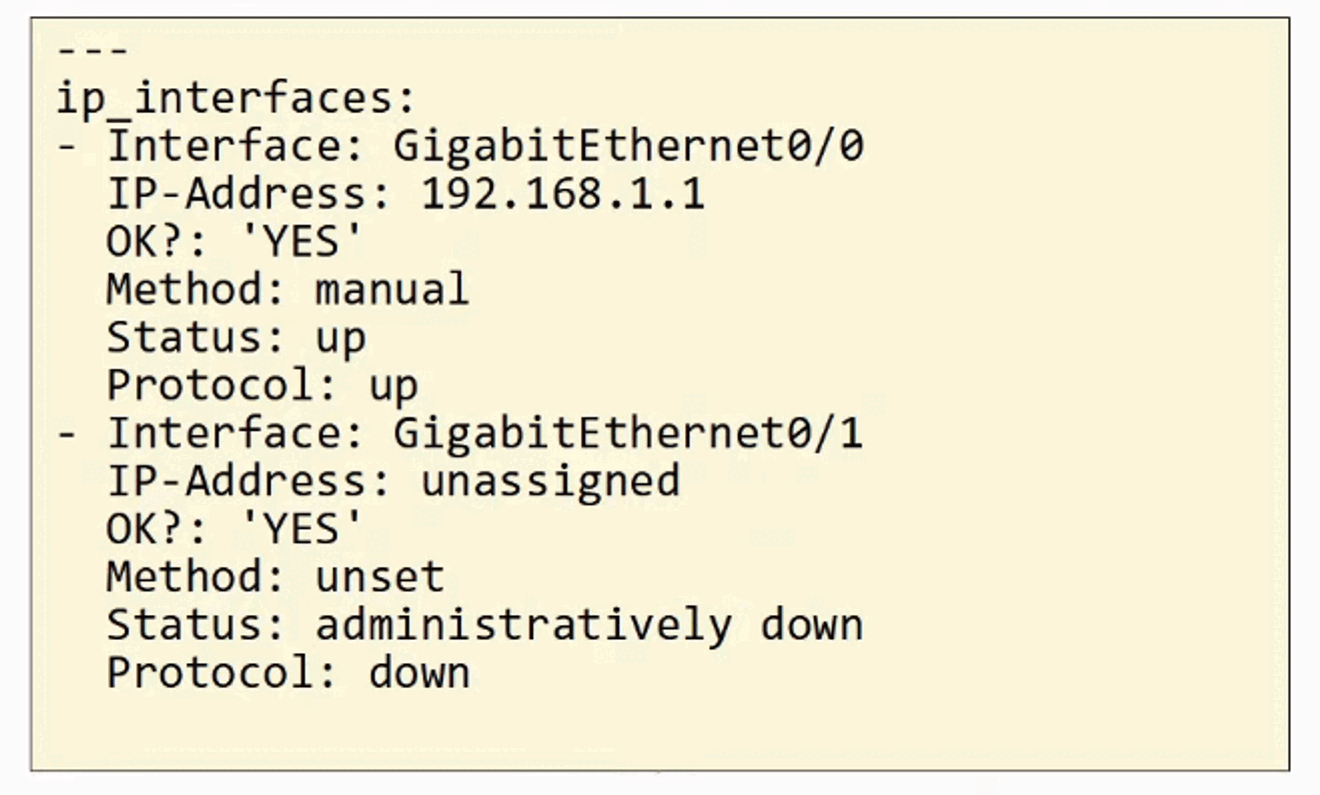
\includegraphics[keepaspectratio,alt={image}]{images/63-json-xml-yaml/img-009.png}}
\end{figure}

COMPARISON BETWEEN JSON and YAML using the same DATA

\begin{figure}
\centering
\pandocbounded{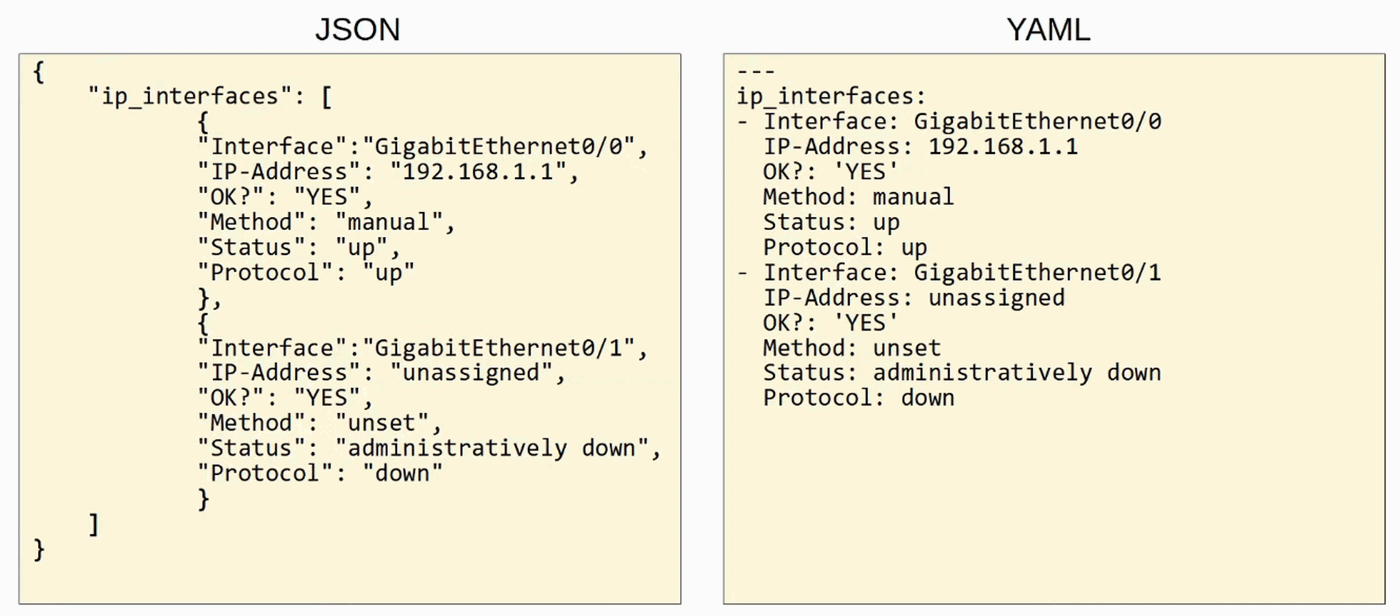
\includegraphics[keepaspectratio,alt={image}]{images/63-json-xml-yaml/img-010.png}}
\end{figure}
